Перспективность данного направления исследований заключается в преимуществах теории нечётких множеств при обработке нечётких данных, которыми изобилует реальная практика разработки ПО в сфере аутсорсинга. Действительно, характерными чертами процесса проектирования и разработки программного обеспечения являются:
\begin{itemize}
  \item относительная уникальность разрабатываемого проекта~--- у некоторых участников может быть опыт участия в схожих проектах, однако он нивелируется тем, что остальная часть команды обычно впервые сталкивается с конкретной задачей автоматизации в некоторой предметной области;
  \item частое отсутствие полных требований к программному продукту либо необходимых для разработки ресурсов (согласованные и утверждённые дизайны, переводы и т.д.);
  \item разный уровень подготовки членов команды разработчиков;
  \item возможность изменения списка работ на поздних стадиях разработки~--- либо увеличение списка требований к продукту, либо его сокращение с целью ускорить разработку и приурочить выпуск готового продукта к некоторому событию;
  \item бюрократическая составляющая~--- затягивание сроков разработки из-за проблем в согласовании изменений или списка работ.
\end{itemize}

В связи с~этим в настоящее время применяемые при планировании разработки ПО методы в основном являются неформальными и базируются на использовании мнений нескольких экспертов. Эксперты, производящие первоначальную оценку проекта, обычно знают о вышеперечисленных потенциальных рисках и~потому стараются учесть все риски в самих временных оценках. Чаще всего применяется вариант интервальной неопределённости, т.\,н. <<вилка>>~--- оценка наиболее пессимистичного и наиболее оптимистичного вариантов разработки. Однако у этого варианта есть несколько существенных недостатков:
\begin{itemize}
  \item обычно заказчики ориентируются на нижнюю границу оценки и не уточняют список потенциальных факторов риска, которые приводят к достижению верхней границы интервала, при этом вынуждая руководителя проекта надавливать на экспертов с целью получения более оптимистичной и точной оценки;
  \item существует негласное правило <<умножения на три>>, которое применяется руководителем проекта при анализе оценок, полученных от экспертов: для каждого этапа проекта из полученных оценок выбирается самая пессимистичная и утраивается~--- в результате неопределённость учитывается дважды; 
  \item эксперт, коим обычно является инженер-программист, исходит из своего опыта и оценки собственной производительности, поэтому оценка может оказаться чрезмерно персонализированной~--- другой исполнитель задания просто не успеет выполнить запланированные работы в срок.
\end{itemize}

В связи с этим логичным выглядит получение оценок в виде нечётких треугольных чисел, поскольку эксперт на основании своего опыта может оценить, сколько времени обычно занимает некоторый этап разработки, и сколько времени он занимал в наилучшем и наихудшем случаях. Учитывая общую склонность инженеров-программистов к пессимистическому оцениванию времени разработки, оценки обычно получаются асимметричными. Применение к оценкам преобразования $L$ позволяет получить модифицированные значения оценок, носители которых могут быть в дальнейшем интерпретированы как нечёткие интервалы, а тип ($LL$ или $RR$)~--- как степень пессимизма или оптимизма. 

Рассмотрим следующий случай. В фирму по разработке программного обеспечения обращается заказчик с просьбой оценить срок и примерную стоимость реализации комплексного решения~--- веб-портала и двух мобильных приложений под наиболее популярные платформы~--- приуроченного к празднованию круглой даты одного из государственных праздников. Для оценки продолжительности проекта собирается команда экспертов, состоящая из руководителя проекта, графического дизайнера, разработчика серверных приложений и двух разработчиков мобильных приложений. Требуется предоставить заказчику <<вилку>> по времени и указать возможные факторы риска незавершения проекта в срок.

В~cтандартный процесс оценивания проекта, состоящий из этапов идентификации операций, построения их взаимосвязей, оценки их продолжительностей и расчёта общего времени проекта, вносятся некоторые изменения. После идентификации операций строится т.\,н. вершинный граф проекта~\cite{Eddous, Taha_Operation_Research}, в котором операции представляются вершинами графа, а дугами показаны их зависимости друг от друга. Построение вершинного графа занимает гораздо меньшее время ввиду отсутствия в нём проблемы фиктивных стрелок, однако для решения задачи планирования лучше подходит стрелочный граф~--- именно на такое представление проекта рассчитаны методы, описанные в главе~\ref{chapter3}. Решить это противоречие позволяет преобразование вершинного графа в стрелочный~\cite{VSU-5y}. В~основу алгоритма преобразования положены следующие правила построения стрелочного графа, описанные в~\cite{Eddous, Taha_Operation_Research}.
\begin{enumerate}
\label{Taha:ConversionRules}
  \item Каждый процесс в проекте представляется только одной дугой.
  \item Каждый процесс идентифицируется двумя концевыми узлами.
  \item Для поддержкания правильных отношений предшествования при включении в сеть любого процесса, необходимо идентифицировать, какой процесс непосредственно предшествует текущему, какой должен выполняться после заверения текущего и какой выполняется параллельно с текущим. В результате идентификации соседних процессов принимается решение о том, требуется ли включить в сеть фиктивные операции для правильного отображения последовательности выполнения задач.
\end{enumerate}

Ниже описана последовательность шагов по преобразованию вершинного графа в стрелочный~\cite{VSU-5y}. $d_i^-$ обозначает число входящих в вершину $v_i$ дуг, $d_i^+$~--- число исходящих, а сумма этих значений равна степени вершины $d_i=d_i^-+d_i^+$.
\begin{enumerate}
\label{ConversionAlgo}
	\item Топологическая сортировка исходного вершинного графа для определения порядка следования операций и начальных вершин графа.
	\item \label{question:veer} Создание начального узла стрелочного графа и исходящих из него дуг-операций. Для этого из исходного вершинного графа $ G_v = (V_v,E_v)$ выбираются те вершины, у которых нет входящих в них стрелок, т.е. все $v_i \in V_v: d_{v_i}^-=0$. Для этих $N$ операций в новом стрелочном графе создаётся $N+1$ вершина, одна из которых будет общей начальной вершиной для всех стрелок. В итоге получается <<веер>> из вершин, изображённый на рисунке~\ref{fig:graph-transform-source}.
	\begin{figure}[h!]
		\centering
		{
			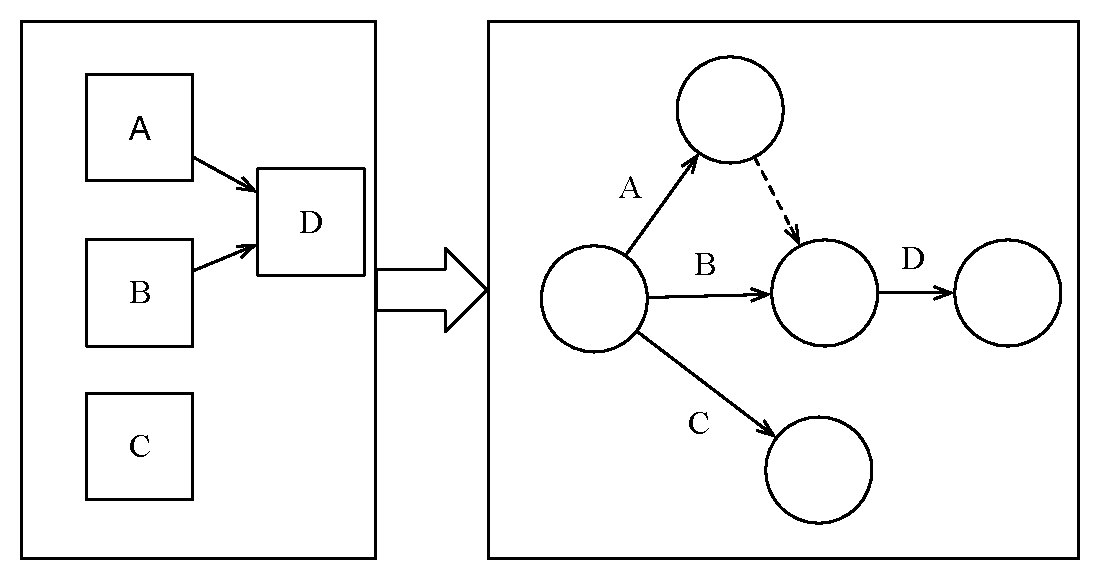
\includegraphics[width=0.9\textwidth]{graph-transform-source}
		}
		\caption{Преобразование начальных операций проекта}
		\label{fig:graph-transform-source}
	\end{figure}
	\item Поочередное добавление оставшихся операций. Для операций, которые ещё не были добавлены в граф, возможны следующие варианты:
	\begin{enumerate}
		\item Добавляемой операции непосредственно предшествует ровно одна операция. В этом случае конечная вершина стрелки, соответствующей непосредственно предшествующей операции, является начальной для новой стрелки. Пример изображён на рисунке~\ref{fig:graph-transform-middle}~--- операции $I$ непосредственно предшествует только одна операция  $G$.
		\begin{figure}[h!]
			\centering
			{
				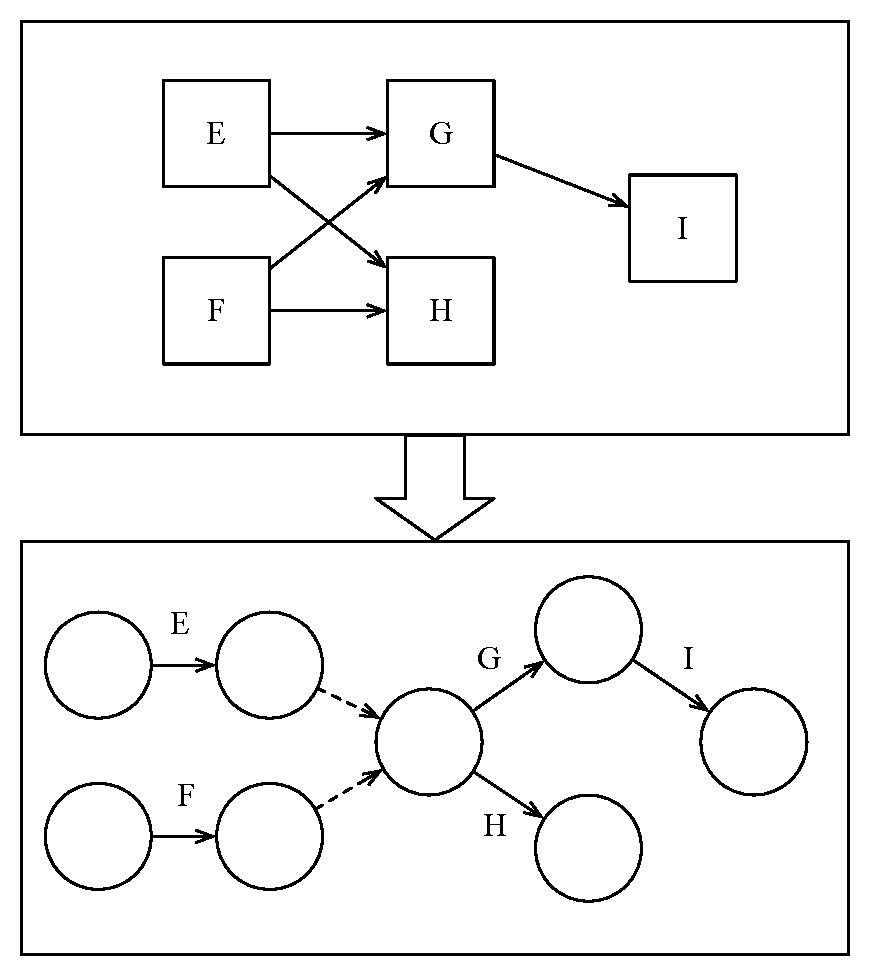
\includegraphics[width=0.75\textwidth]{graph-transform-middle}
			}
			\caption{Дальнейшее добавление операций}
			\label{fig:graph-transform-middle}
		\end{figure}
		\item Добавляемой операции непосредственно предшествует несколько операций. В этом случае в вершинном графе ищутся другие операции, которые ещё не были добавлены в новый граф, и у которых тот же набор непосредственно предшествующих операций. Если таких операций оказалось несколько, то выполняются действия, аналогичные описанным в~п.~\ref{question:veer}, и добавляются фиктивные дуги, соединяющие конечные вершины предшествующих операций и начальную вершину "веера". На рисунке~\ref{fig:graph-transform-middle} у вершин $G$ и $H$ как раз одинаковые непосредственно предшествующие вершины $E$ и $F$. Иначе создаётся единственная дуга, начало которой соединяется фиктивными дугами с концами непосредственно предшествующих вершин.
	\end{enumerate}
	\item Соединение концов завершающих дуг в одной вершине. Для этого в созданном стрелочном графе выбираются все вершины $v_i \in V$: $d_{v_i}^+=0$, и создаётся единственная конечная вершина. Все дуги, входящие в вершины $v_i$, перенаправляются на новую вершину, а старые конечные вершины удаляются. Пример такого преобразования можно увидеть на рисунке~\ref{fig:graph-transform-sink}
	\begin{figure}[h!]
		\centering
		{
			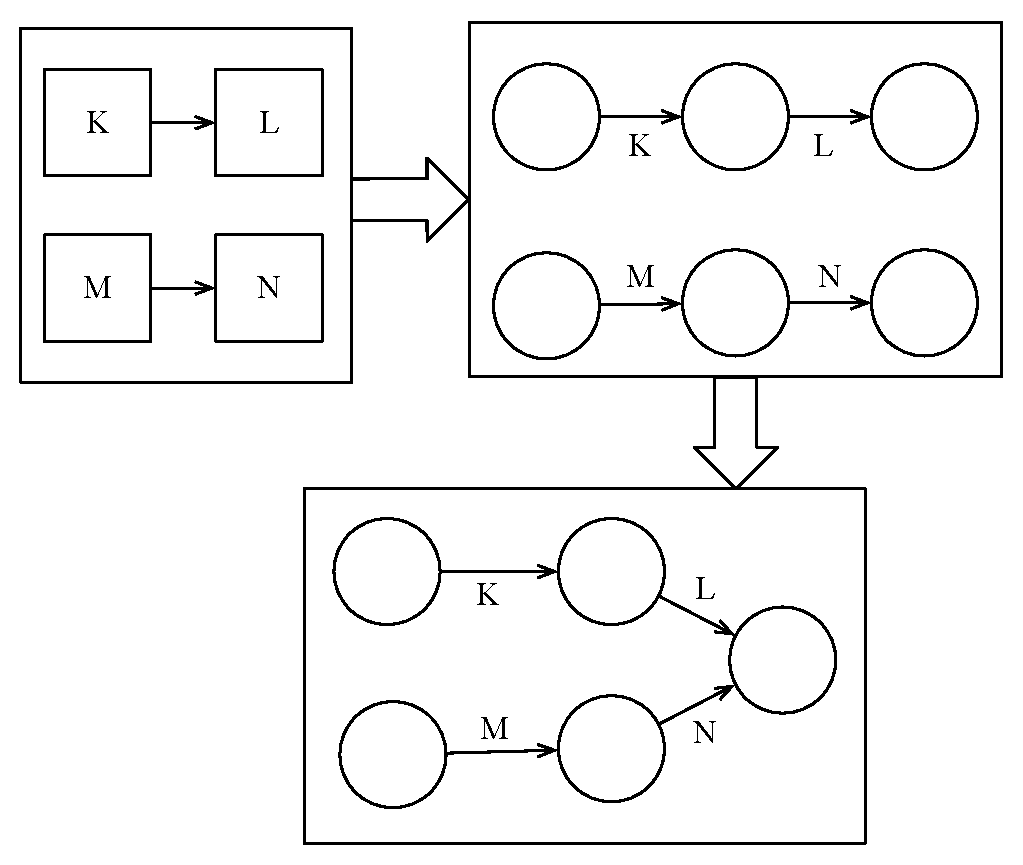
\includegraphics[width=0.9\textwidth]{graph-transform-sink}
		}
		\caption{Соединение конечных дуг в одной вершине}
		\label{fig:graph-transform-sink}
	\end{figure}
	\item Упрощение графа с помощью удаления фиктивных дуг. На последнем этапе происходит уменьшение числа дуг в соответствие с правилами, описанными на стр.~\pageref{Taha:ConversionRules}. В построенном стрелочном графе $G_S$ выбираются все фиктивные дуги $e_{F_i}=\left(v_{S_i}; v_{E_i}\right)$; затем для каждой $e_{F_i}$ происходит проверка, не используется ли она для обозначения параллельно выполняющихся процессов. Проверяются следующие условия:
	\begin{itemize}
		\item из начальной вершины $v_{S_i}$ дуги $e_{F_i}$ не выходит никаких других дуг, кроме самой $e_{F_i}$;
		\item $V_P(v_{S_i}) \bigcap V_P(v_{E_i}) = \varnothing $ и $V_S(v_{S_i}) \bigcap V_S(v_{E_i}) = \varnothing$, где $V_P(v_i), V_S(v_i)$~--- множества вершин, непосредственно предшествующих вершине $v_i$ и непосредственно следующих за $v_i$ соответственно.
	\end{itemize}
	 Если оба этих условия выполняются, то можно исключить проверенную дугу из графа, объединяя её начальную и конечную вершины.
\end{enumerate}

После построения сетевого графика, эксперты-разработчики формулируют интервальные оценки $\left[ x_i^L, x_i^R \right]$ для всех операций проекта, но при этом их дополнительно просят указать наиболее возможный, с их точки зрения, срок выполнения операции $m_i$. Вместе эти три параметра используются для формирования нечёткой треугольной оценки $\tau_i=\left \langle x_i^L, m_i, x_i^R \right \rangle = \left \langle m_i, m-x_i^L, x_i^R-m \right \rangle$. Полученные нечёткие оценки $\tau_i$ в дальнейшем будут использованы для расчёта общего времени выполнения проекта и поиска критического пути.

Критический путь и~время выполнения проекта находятся с~помощью модификации классического алгоритма Дейкстры. Возможны два варианта поиска критического пути: двухточечный, когда расчёты выполняются дважды~--- при $\alpha=0$ и $\alpha=1$, и $\alpha$-уровневый, при котором задаётся число уровней поиска $q$, и~алгоритм для чёткого случая выполняется $q$ раз на~различных $\alpha$-уровнях, расстояние между которыми равно $\displaystyle \frac{1}{q}$. В~первом случае модифицированное нечёткое время выполнения восстанавливается согласно~\eqref{eq:isomorphic-field}, а во втором на выходе получается нечёткая величина с дискретной функцией принадлежности, которую также в большинстве случаев удаётся интерполировать линейной зависимостью.

Найденные общее нечёткое время выполнения проекта и критические операции могут быть представлены заказчику как <<вилка>> и потенциально рискованные операции соответственно.

Перейдём к~описанию программного средства, призванного автоматизировать процесс получения нечёткой временной оценки проекта и~соответствующий ей критический путь.
